\documentclass{article}
\usepackage[utf8]{inputenc}
\usepackage{multicol}
\usepackage[formats]{listings}
\lstloadaspects{formats}
\usepackage{verbatim}
\usepackage{color}
\usepackage{geometry}
\usepackage{float}
\usepackage{amsmath}
\usepackage{caption}
\usepackage{pdflscape}
\usepackage{caption}
\usepackage[font={color=black},figurename=Fig.,labelfont={it}]{caption}
\usepackage{hyperref}
\setlength{\belowcaptionskip}{-10pt}
\setlength{\abovecaptionskip}{-30pt}
\floatstyle{boxed} 
\restylefloat{figure}
\usepackage{graphicx}
\definecolor{codegreen}{rgb}{0,0.6,0}
\definecolor{codegray}{rgb}{0.5,0.5,0.5}
\definecolor{codepurple}{rgb}{0.58,0,0.82}
\definecolor{backcolour}{rgb}{0.95,0.95,0.92}
\lstdefinestyle{mystyle}{
	backgroundcolor=\color{backcolour},   
	commentstyle=\color{codegreen},
	keywordstyle=\color{blue},
	numberstyle=\tiny\color{codegray},
	stringstyle=\color{codepurple},
	basicstyle=\footnotesize,
	breakatwhitespace=false,         
	breaklines=true,                 
	captionpos=b,                    
	keepspaces=true,                 
	numbers=left,                    
	numbersep=5pt,                  
	showspaces=false,                
	showstringspaces=false,
	showtabs=false,                  
	tabsize=2
}
\lstset{style=mystyle}
\title{Data Mining\\
		Home work 11\\ML, Clustering, projects... }
\author{Aqeel Labash\\ \textbf{Lecturer:} Jaak Vilo}
\date{21 April 2016}
\geometry{
	a4paper,
	total={170mm,257mm},	
	left=10mm,
	top=5mm,
}
\begin{document}
	\maketitle
\section*{First Question}
For this question I simply created a new point depending on the mean value of all \(Xs ,Ys\) and then calculated the distance between all the points and that point as the \(Z\) value. Here is the code I used : 
\begin{lstlisting}[language=Python]
import pandas as pd
import numpy as np
get_ipython().magic(u'matplotlib inline')
import matplotlib.pyplot as plt
from IPython.display import display, HTML
from mpl_toolkits.mplot3d import Axes3D
from matplotlib import cm

data =pd.read_csv('Linear.csv',sep=',')
plt.plot(data[data.Class==1].X, data[data.Class==1].Y, 'ro')
plt.plot(data[data.Class==0].X, data[data.Class==0].Y, 'bo')
(mX,mY) = (np.mean(data.X),np.mean(data.Y))
plt.plot(mX,mY,'go')
plt.axis([min(data.Y)-1, max(data.X)+1, min(data.Y)-1, max(data.Y)+1])
plt.show()

# #The three levels is :
# - X
# - Y
# - Z :distance from the mean point
lst =[]
for i in range(len(data.X)):
    lst.append(np.linalg.norm(np.array((data.X[i],data.Y[i]))-np.array((mX,mY))))

data['Z'] = pd.Series(np.array(lst), index=data.index)

fig = plt.figure()
ax = fig.add_subplot(111, projection='3d')
ax.scatter(data[data.Class==1].X, data[data.Class==1].X, data[data.Class==1].Z, c='r', marker='o')
ax.scatter(data[data.Class==0].X, data[data.Class==0].X, data[data.Class==0].Z, c='b', marker='o')

xx, yy = np.meshgrid(range(6), range(6))
z1 = np.reshape(np.repeat(1.65,36),(6,6))

ax.plot_surface(xx,yy,z1, color='blue',                rstride=3, 
                cstride=3, 
                alpha=0.3,            # transparency of the surface 
                cmap=cm.coolwarm)

ax.set_xlabel('X Label')
ax.set_ylabel('Y Label')
ax.set_zlabel('Z Label')

plt.show()
\end{lstlisting}

The previous code output The following figures : 
\begin{figure}[H]
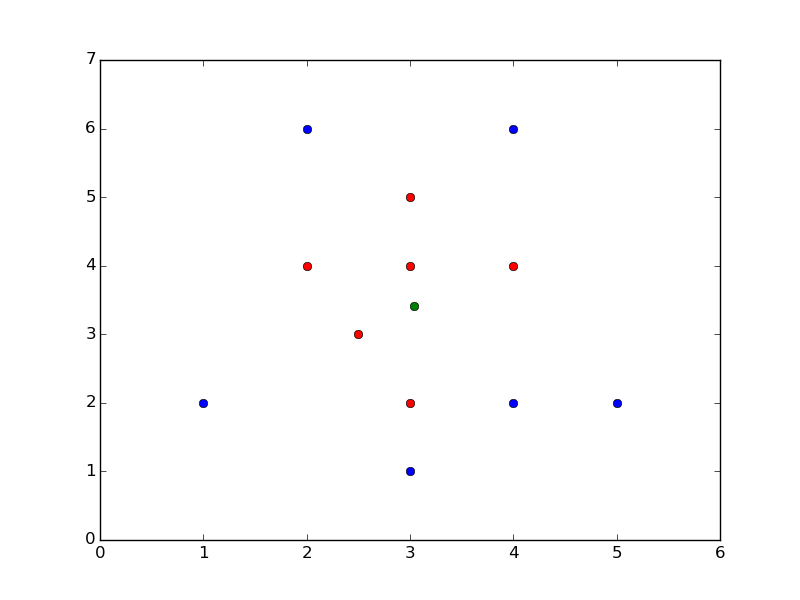
\includegraphics[scale=0.7]{points.png}
\caption{Show the points in the plane with the mean point}
\end{figure}
In the previous figure we can see the green point which represent the mean point between all the points.
\begin{figure}[H]
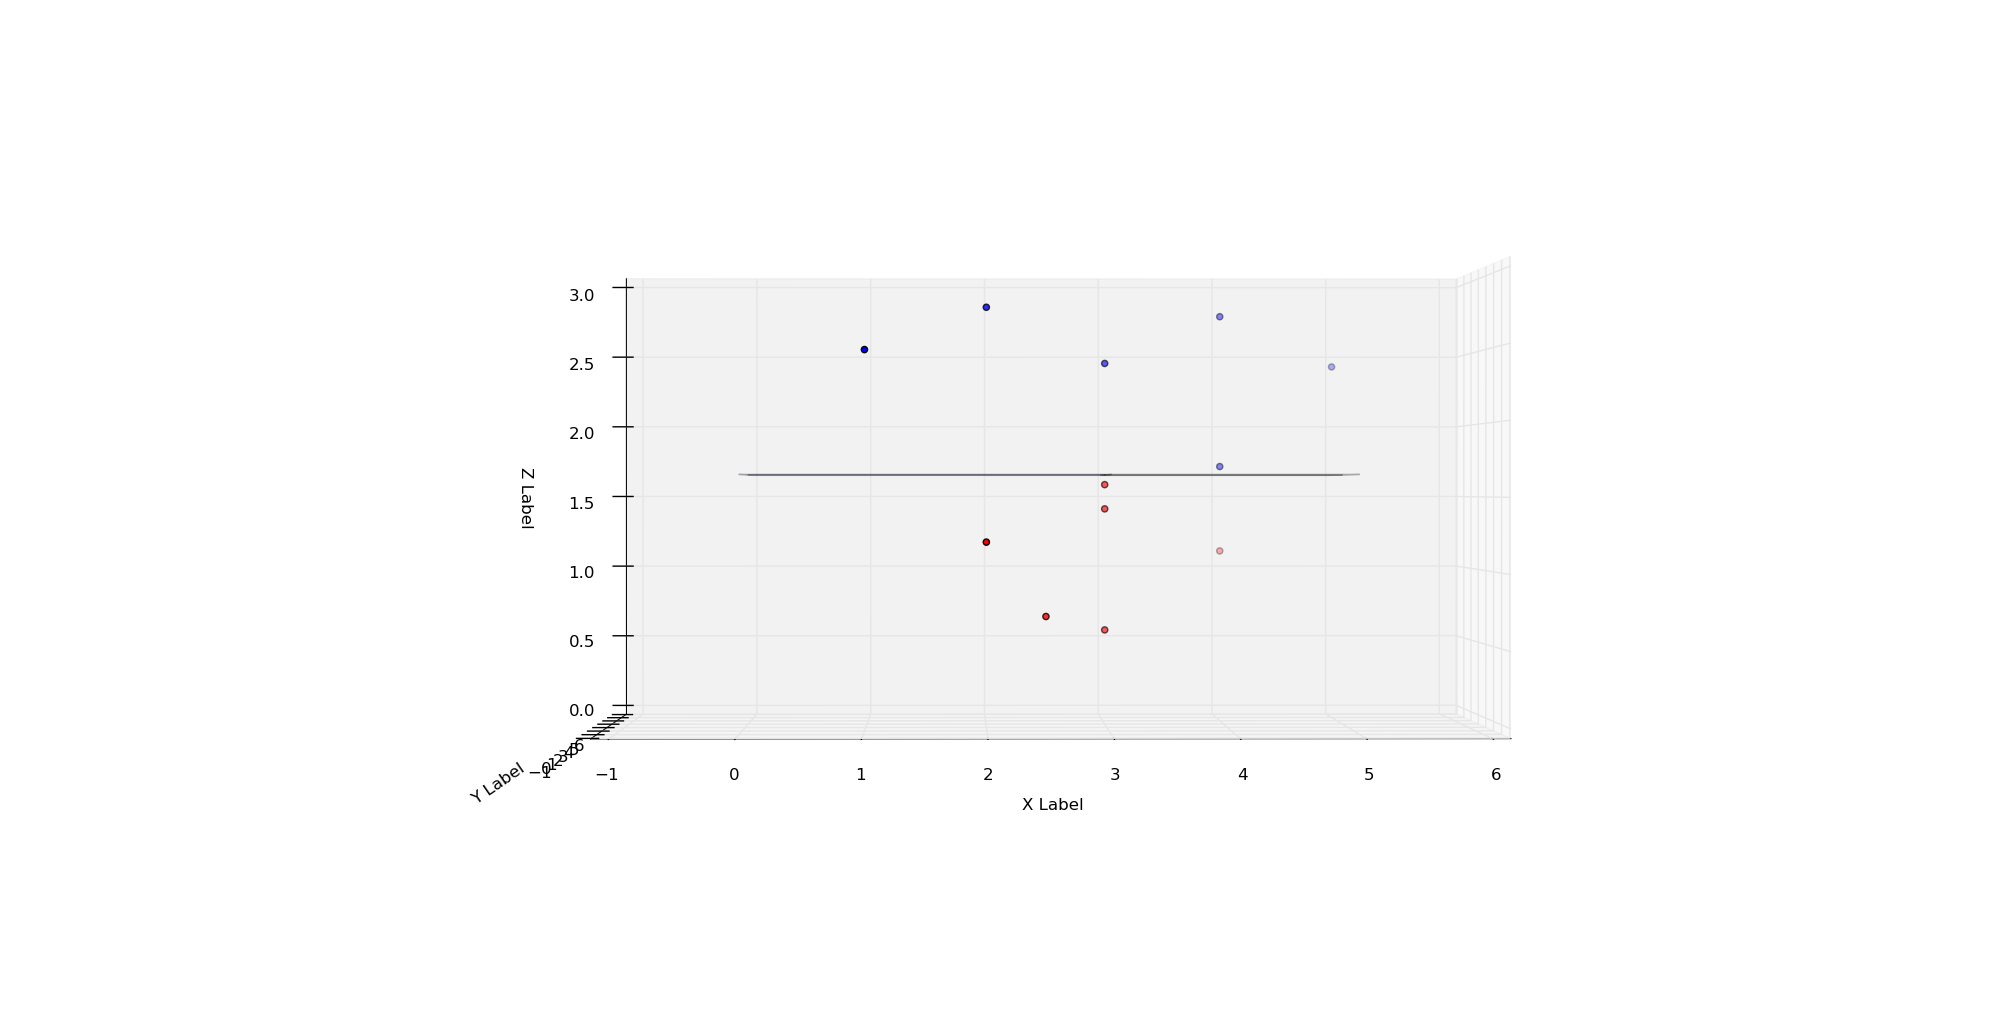
\includegraphics[trim={12cm 5cm 12cm 5cm},clip,scale=0.6]{horizntal.png}
\caption{The hyper plan in 2d prospective}
\end{figure}

\begin{figure}[H]
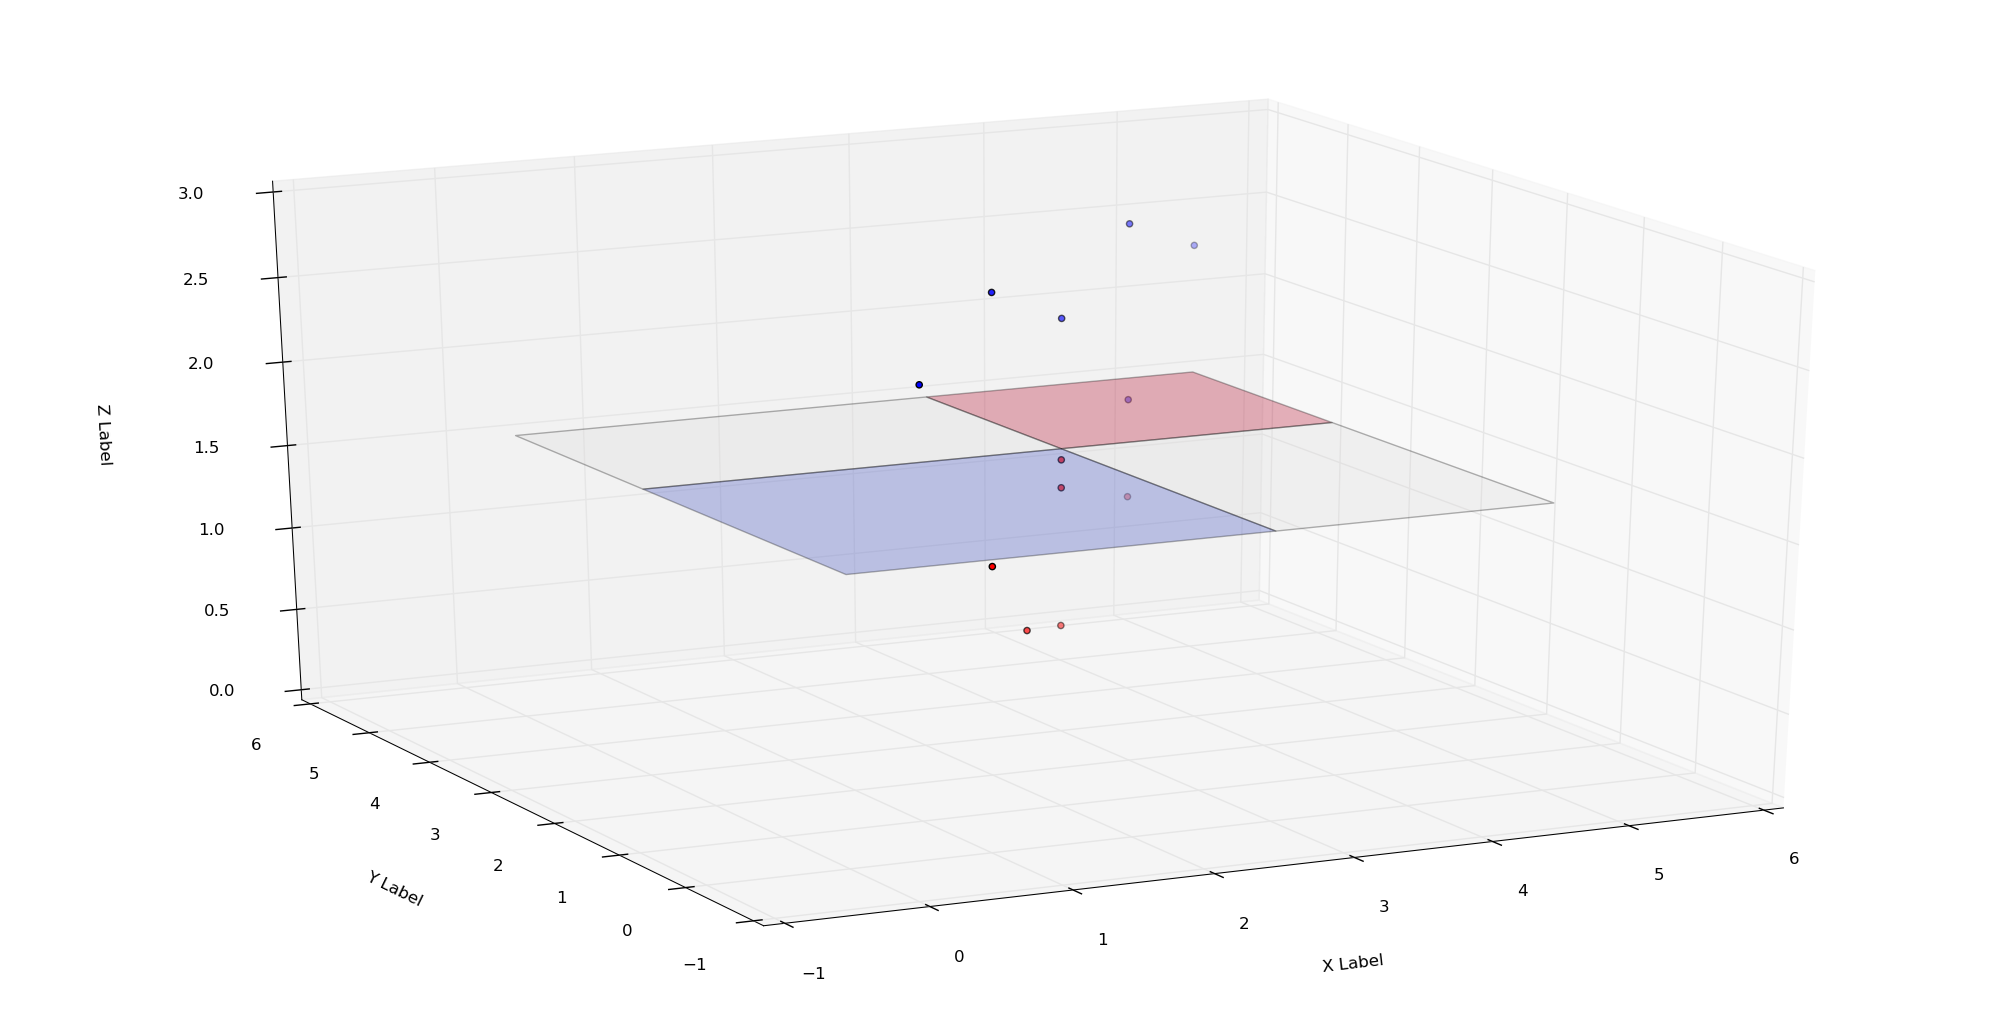
\includegraphics[trim={1cm 0 10cm 2cm},clip,scale=0.4]{3d.png}
\caption{The hyper plane in 3d prospective}
\end{figure}
Please notice that we can add angle to the hyper plane which would give a bigger margin even.
\section*{Second Question}
For this question I used python code to calculate the distances and make things easier (Just to print the distance list and draw a picture of the points). Here is the code : 
\begin{lstlisting}[language=Python]
import pandas as pd
import numpy as np
get_ipython().magic(u'matplotlib inline')
import matplotlib.pyplot as plt
from IPython.display import display, HTML
from mpl_toolkits.mplot3d import Axes3D
from matplotlib import cm
from operator import attrgetter

points = pd.read_csv('Clustering.csv',sep=',')

plt.plot(points.X, points.Y, 'ro')
plt.axis([min(points.X)-1, max(points.X)+1, min(points.Y)-1, max(points.Y)+1])
for i, txt in enumerate(points.index):
    plt.annotate(txt+1, (points.X[i],points.Y[i]))
plt.show()

class Dist:
    def __init__(self,p1indx,p2indx,dist):
        self.p1 = p1indx
        self.p2 = p2indx
        self.dist=dist
distances={}
distancelst = []
for i in range(len(points.index)):
    for j in range(len(points.index)):
        if i==j:
            continue
        if (i,j) not in distances.keys():
            dist = np.linalg.norm(np.array([points.X[i],points.Y[i]])-np.array([points.X[j],points.Y[j]]))
            distances[(i,j)]=dist
            distances[(j,i)]=dist
            distancelst.append(Dist(i,j,dist))

distancelst.sort(key=lambda x: x.dist, reverse=False)

for i in distancelst:
    print i.dist,i.p1+1,i.p2+1
\end{lstlisting}
In the previous code I just calculate the distance between all the points and order them min to max so I can pick what points to connect first.Here is the outcome from the previous code.
\begin{figure}[H]
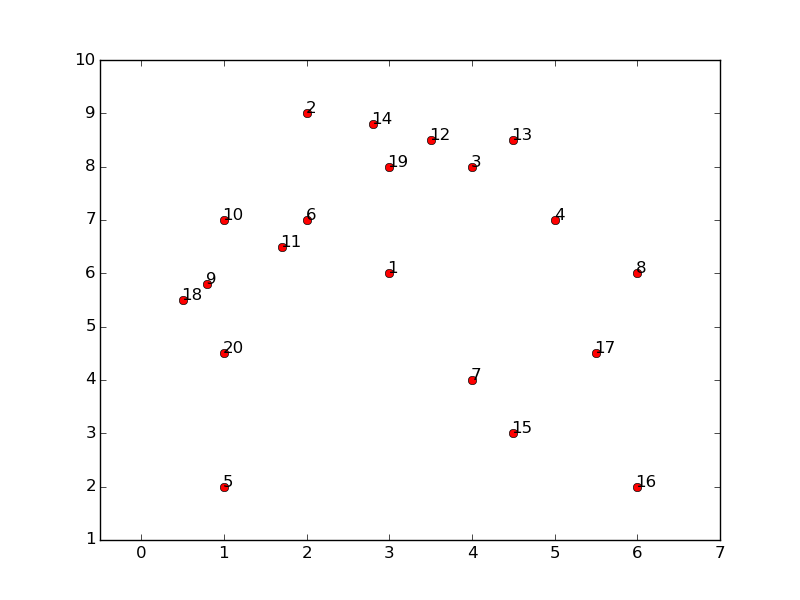
\includegraphics[scale=0.7]{q2points.png}
\caption{Points in the plane numbered}
\end{figure}
The previous code as I said prints the list of ordered points by distance here is the table of it :\\
\begin{tabular}{|c|c|c|c|}
\hline
Distance&Point 1 & Point 2&Notes\\ \hline
0.424264068712&9&18&C1\\ \hline 
 0.583095189485&6&11&C2\\ \hline 
 0.707106781187&3&12&C3\\ \hline 
 0.707106781187&3&13&C3 Extended\\ \hline 
 0.707106781187&12&19&C3 Extended\\ \hline 
 0.761577310586&12&14&C3 Extended\\ \hline 
 0.824621125124&2&14&C3 Extended\\ \hline 
 0.860232526704&10&11&C2 Extended\\ \hline 
 1.11803398875&7&15&C4\\ \hline 
 1.11803398875&18&20&C1 Extended\\ \hline 
 1.1401754251&9&11&C1\&C2 merged\(\rightarrow\) C1\\ \hline 
 1.39283882772&1&11&C1 Extended\\ \hline 
 1.41421356237&3&4&C3 Extended\\ \hline 
 1.41421356237&4&8&C3 Extended\\ \hline 
 1.41421356237&6&19&C1\&C3 merged\(\rightarrow\) C1\\ \hline  
 1.58113883008&7&17&C4 Extended\\ \hline 
 1.58113883008&8&17&C1\&C4 merged\(\rightarrow\) C1\\ \hline 
 1.80277563773&15&16&C1 Extended\\ \hline 
 2.5&5&20&C1 Extended\\ \hline 
\end{tabular}
From the previous table I could see better the shortest distance.And here is what I got on papers:
\begin{figure}[H]
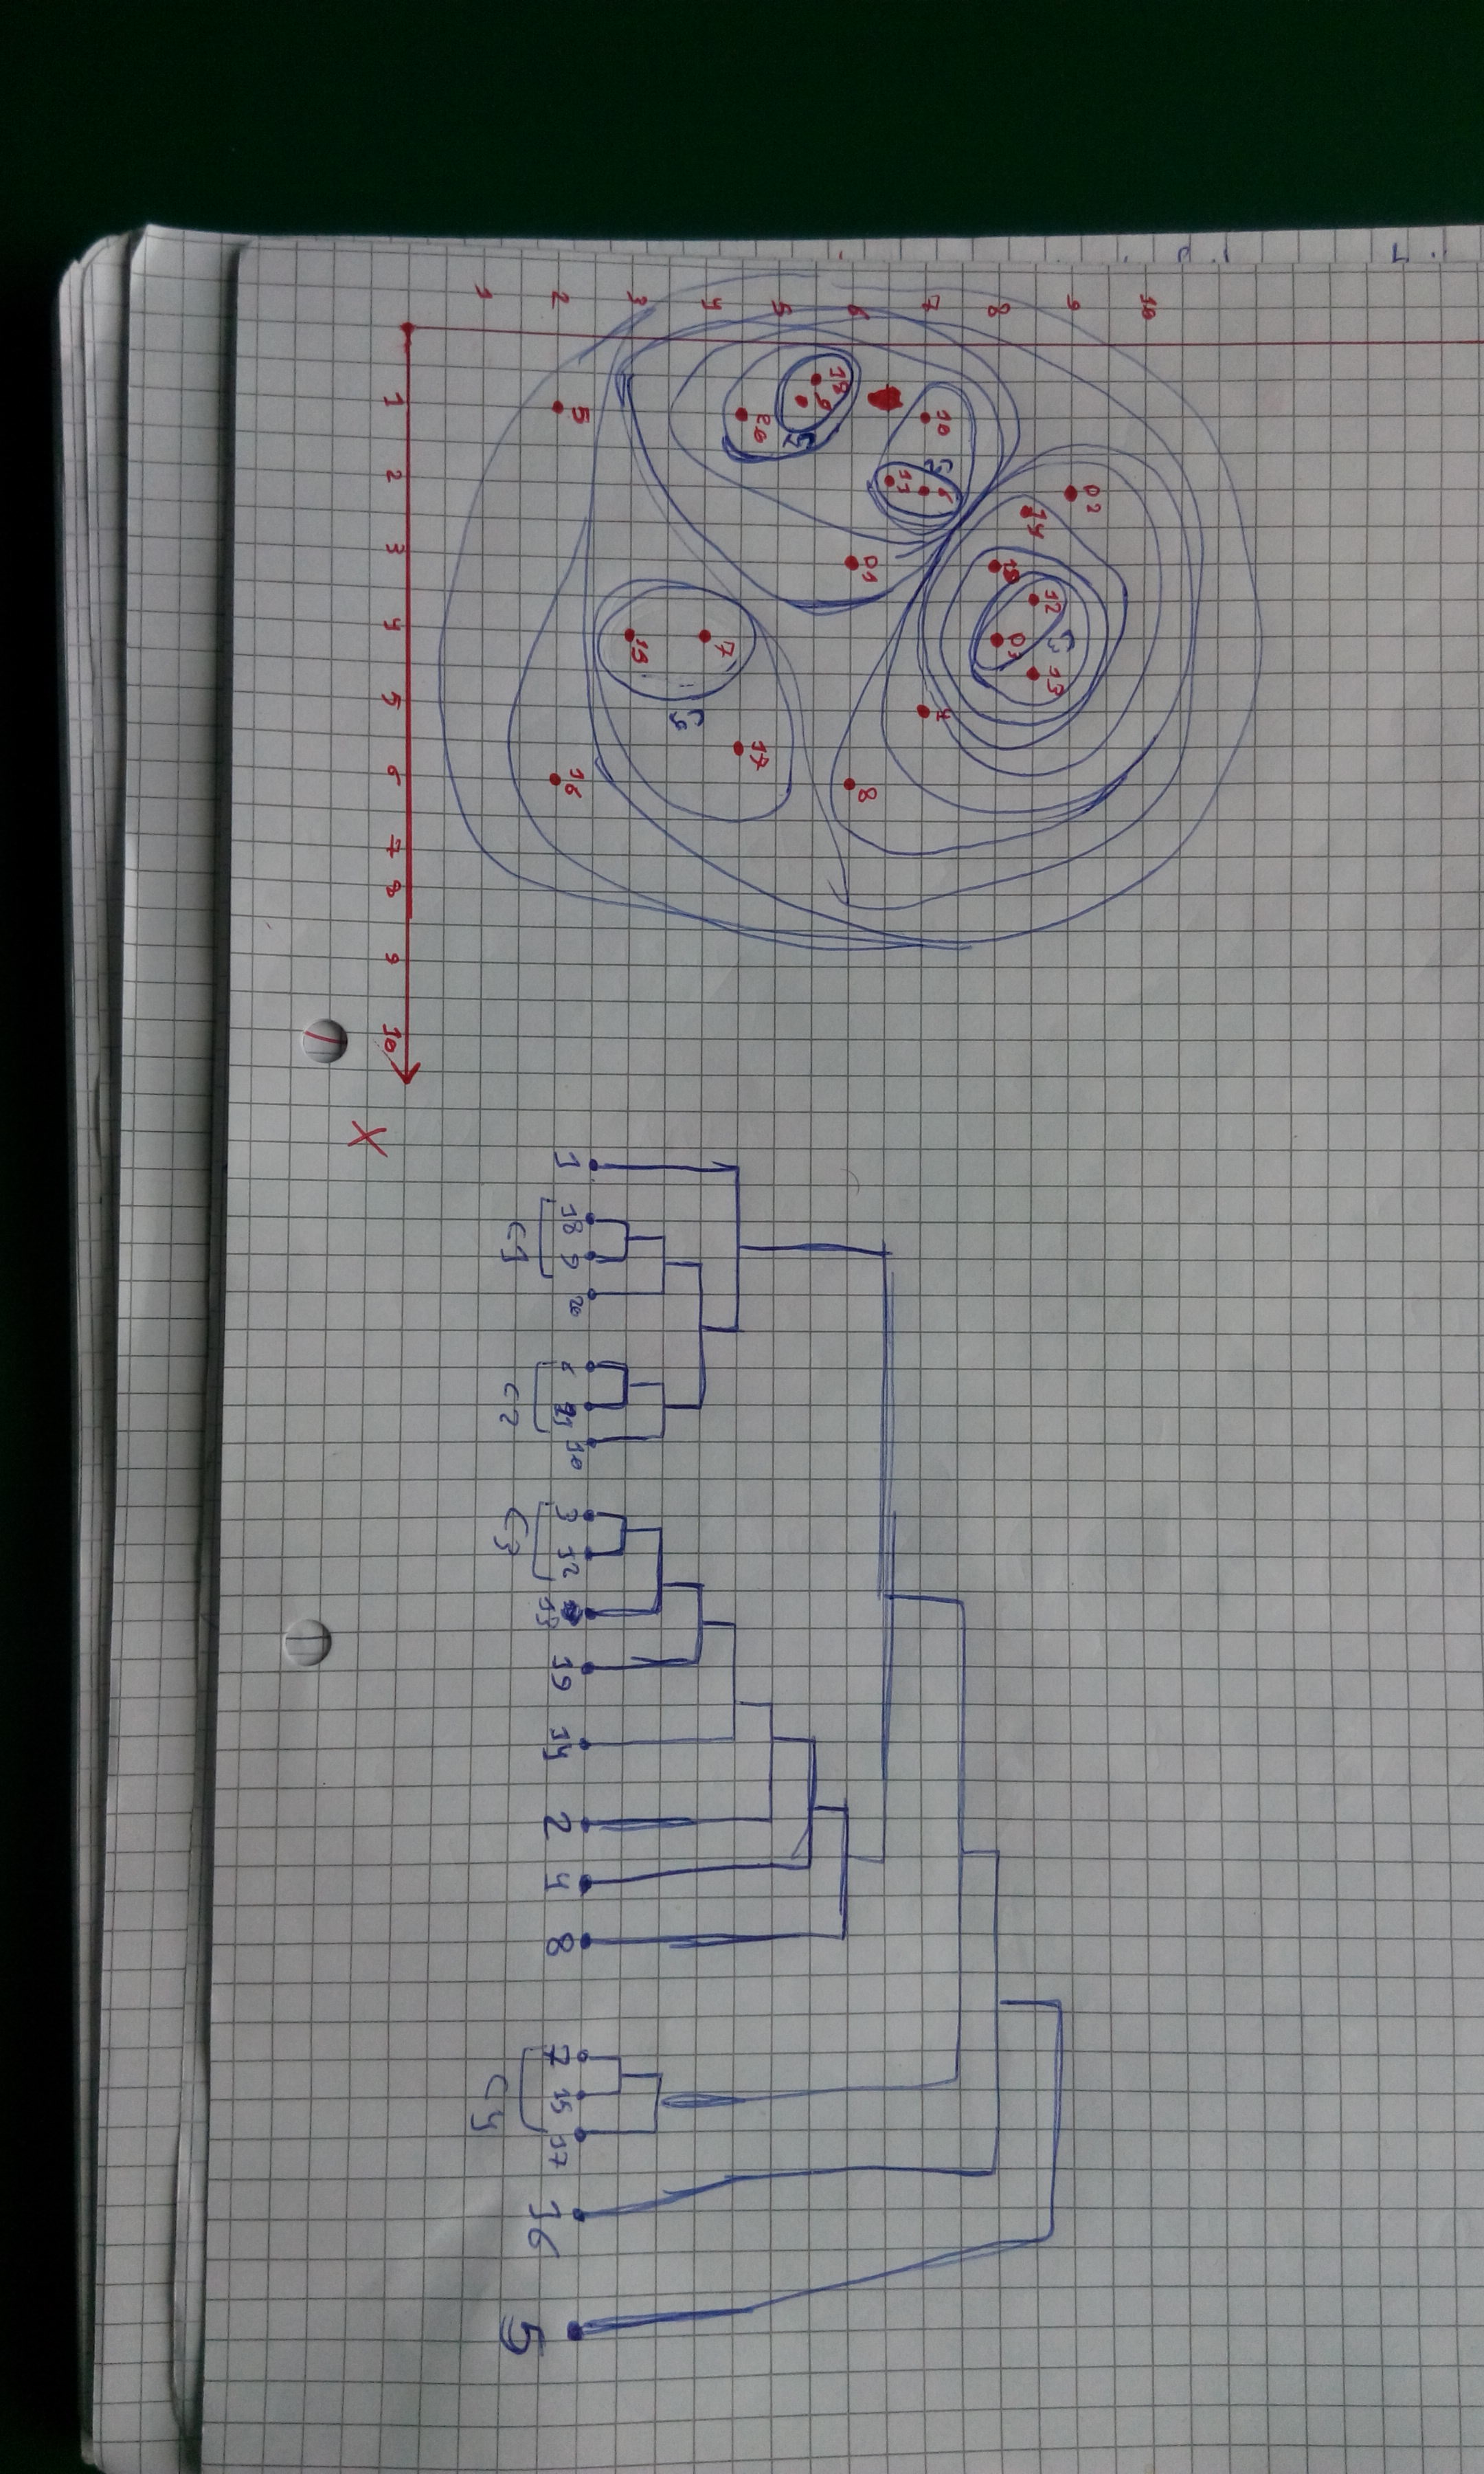
\includegraphics[scale=0.15,angle=90,trim={10cm 5cm 10cm 10cm},clip]{single_link.jpg}
\caption{The clusters build}
\end{figure}
Please notice that the previous plot may not be accurate due to many points (I might mixed some points) but the tree is correct  I believe because  I depended on automated calculation for it.I tried to automate the drawing but didn't continue it not to take more time.
\begin{figure}[H]
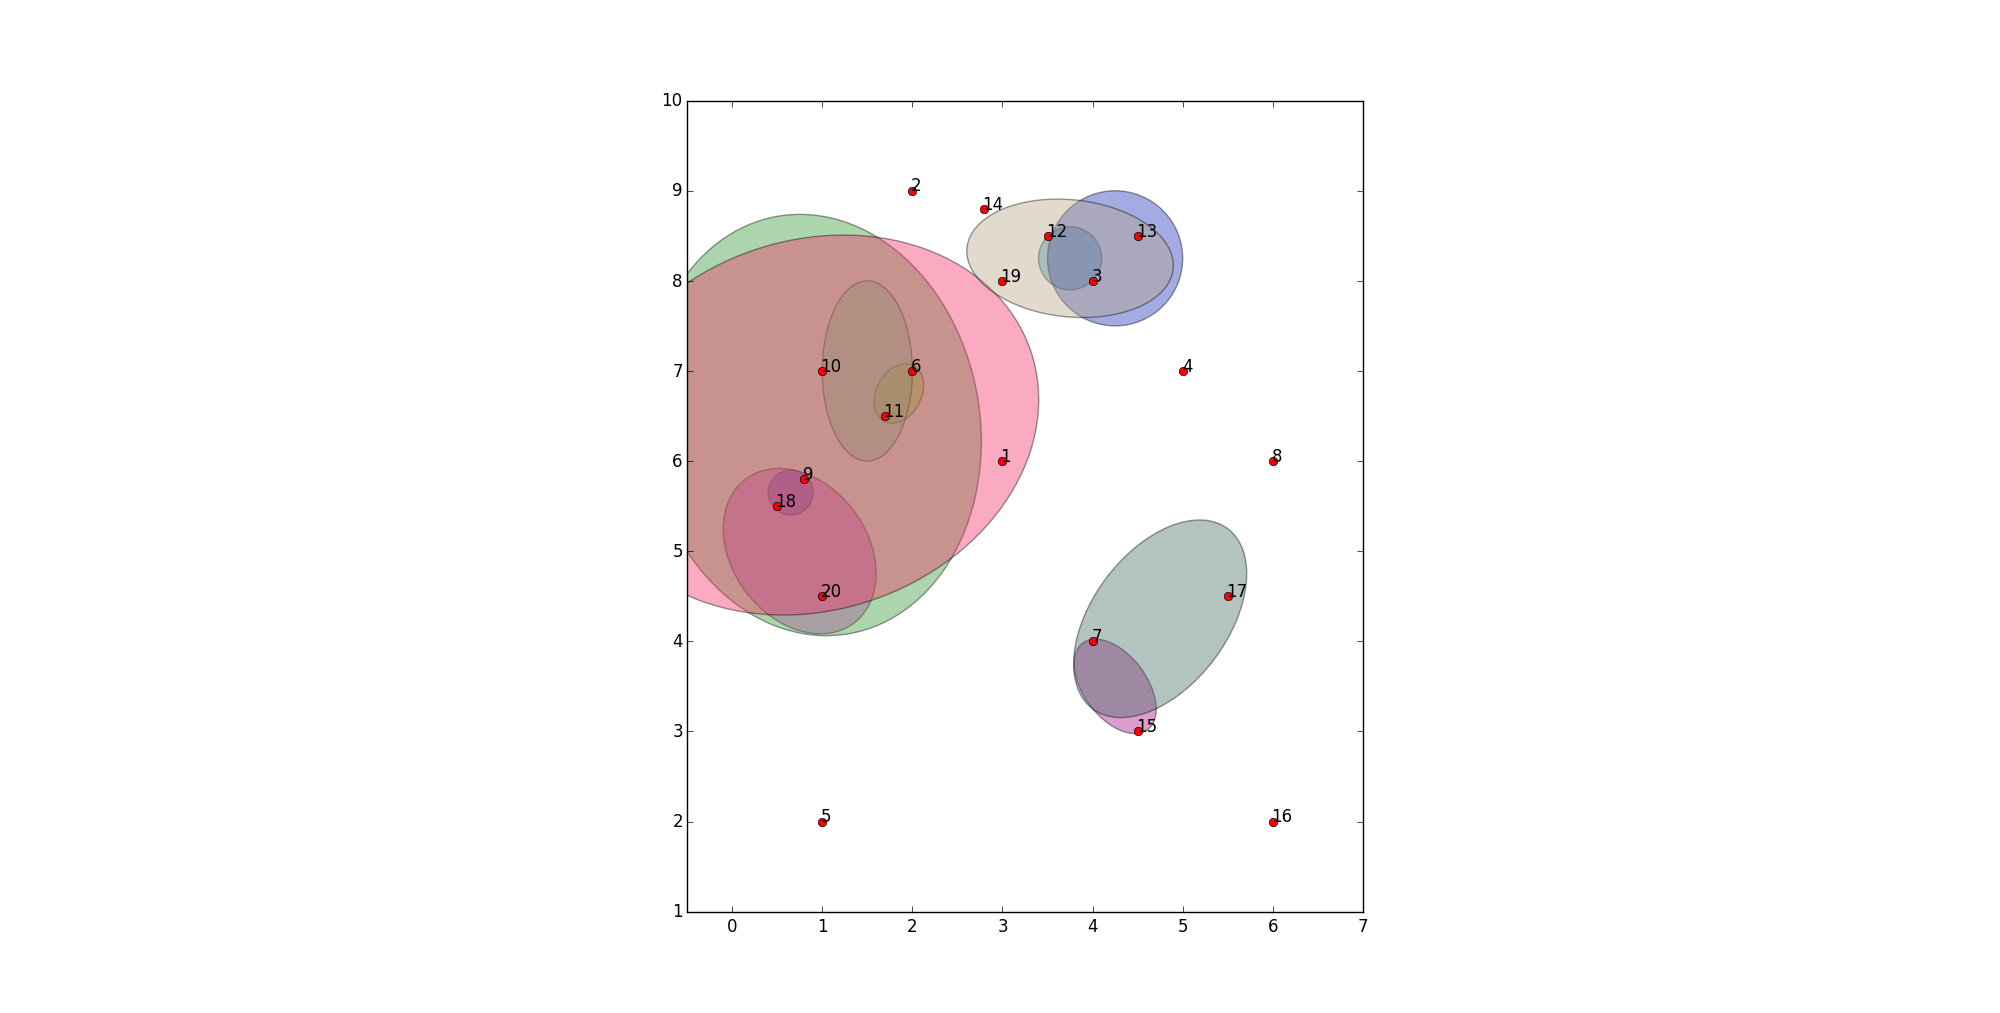
\includegraphics[scale=0.7,trim={15cm 2cm 15cm 2cm},clip]{groups.png}
\caption{Show some groups}
\end{figure}
Now for the \textbf{Complete link}, the first stage is the same when we create join the first clusters (at the beginning  each point is a cluster).And here is the distance table (New one ):\\
\begin{tabular}{|c|c|c|c|}
\hline
Distance&Point 1 & Point 2&Notes\\ \hline
0.424264068712&9&18&C1\\ \hline 
 0.583095189485&6&11&C2\\ \hline 
 0.707106781187&3&12&C3\\ \hline  
 0.824621125124&2&14&C4\\ \hline 
 1.0&3&19&C3 Extended\\ \hline 
 1.0&6&10&C2 Extended\\ \hline 
 1.11803398875&7&15&C5\\ \hline 
 1.3152946438&9&20&C1 Extended\\ \hline 
 1.41421356237&4&8&C6\\ \hline 
 1.58113883008&13&19&C3 Extended\\ \hline 
 1.80277563773&15&17&C5 Extended\\ \hline 
 2.2360679775&1&10&C2 Extended\\ \hline 
 2.2360679775&2&3&C4\&C3 merged \(\rightarrow\)C3\\ \hline 
 2.69258240357&6&20&C1\&C2 merged \(\rightarrow\)C1\\ \hline 
 2.82842712475&7&16&C5 Extended\\ \hline 
 5.0&2&8&C3\&C6 merged \(\rightarrow\)C3\\ \hline 
 5.09901951359&5&6&C1 Expanded\\ \hline 
 7.07106781187&10&16&C1\&C5 merged \(\rightarrow\)C1\\ \hline 
 8.0622577483&2&16&C1\&C3 merged \(\rightarrow\)C1\\ \hline
\end{tabular}
And here is the images:
\begin{figure}[H]
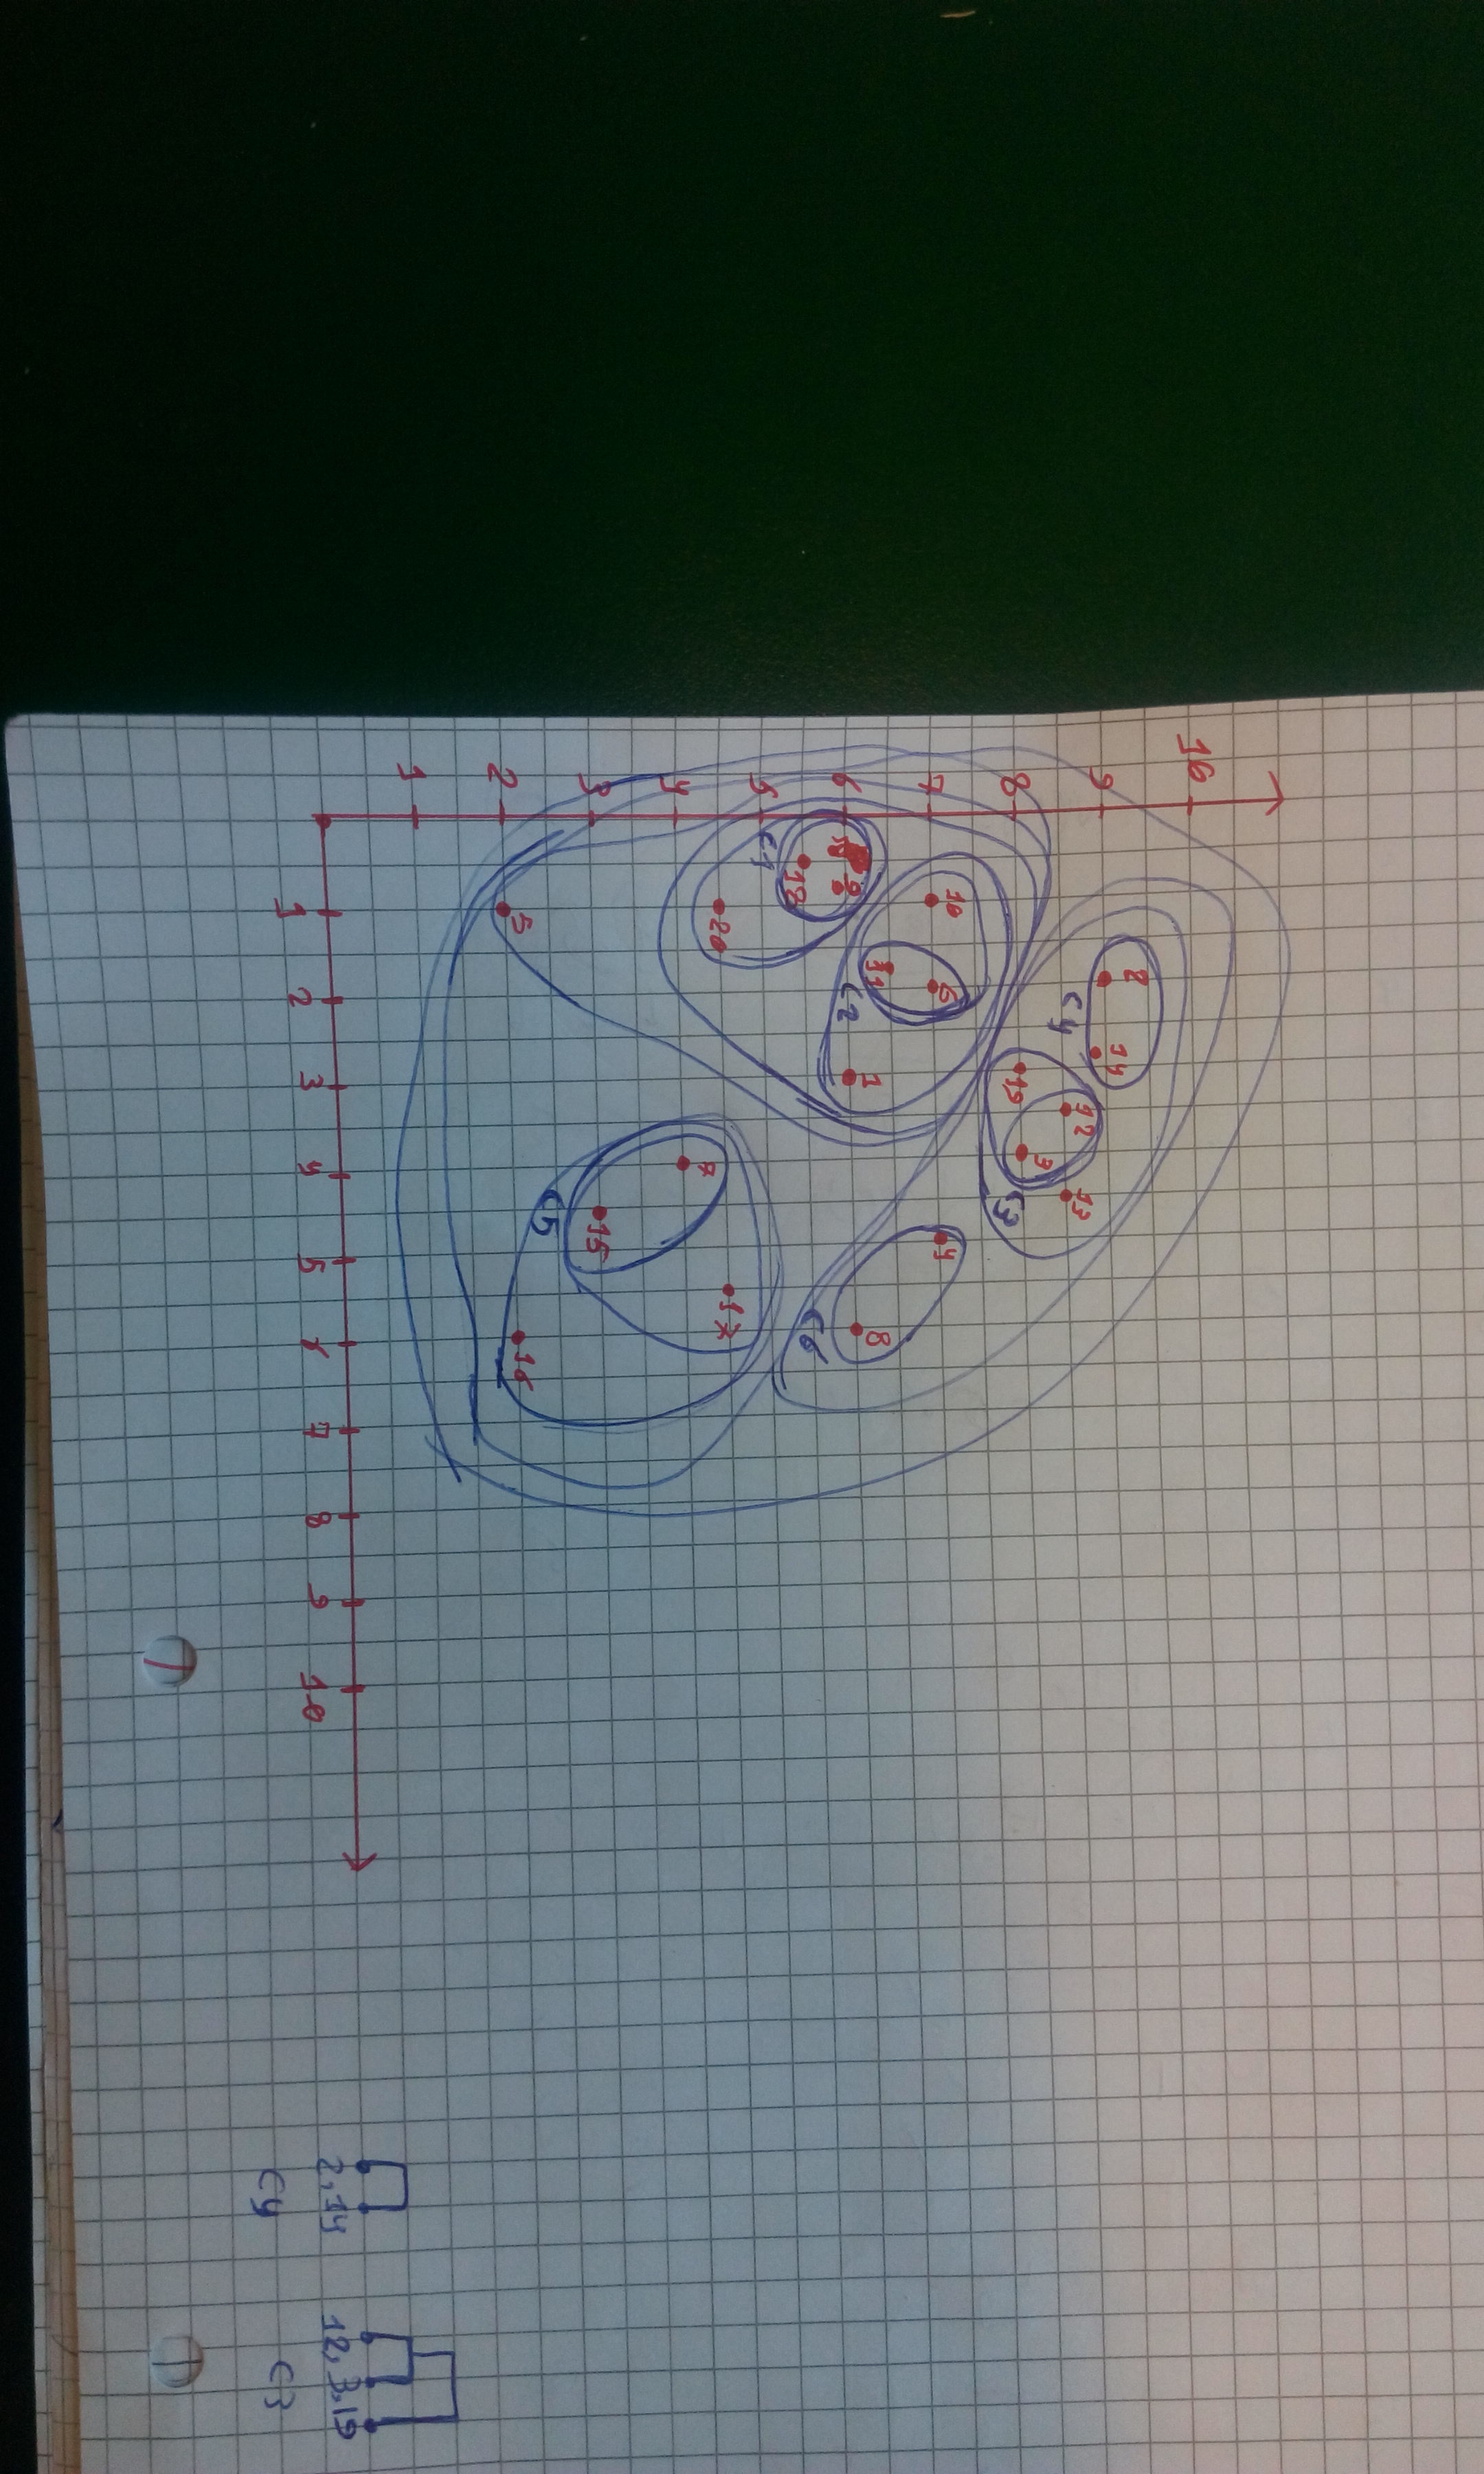
\includegraphics[angle=90,scale=0.25,trim={10cm 30cm 10cm 30cm},clip]{complete_link.jpg}
\caption{Joining points map}
\end{figure}
\begin{figure}[H]
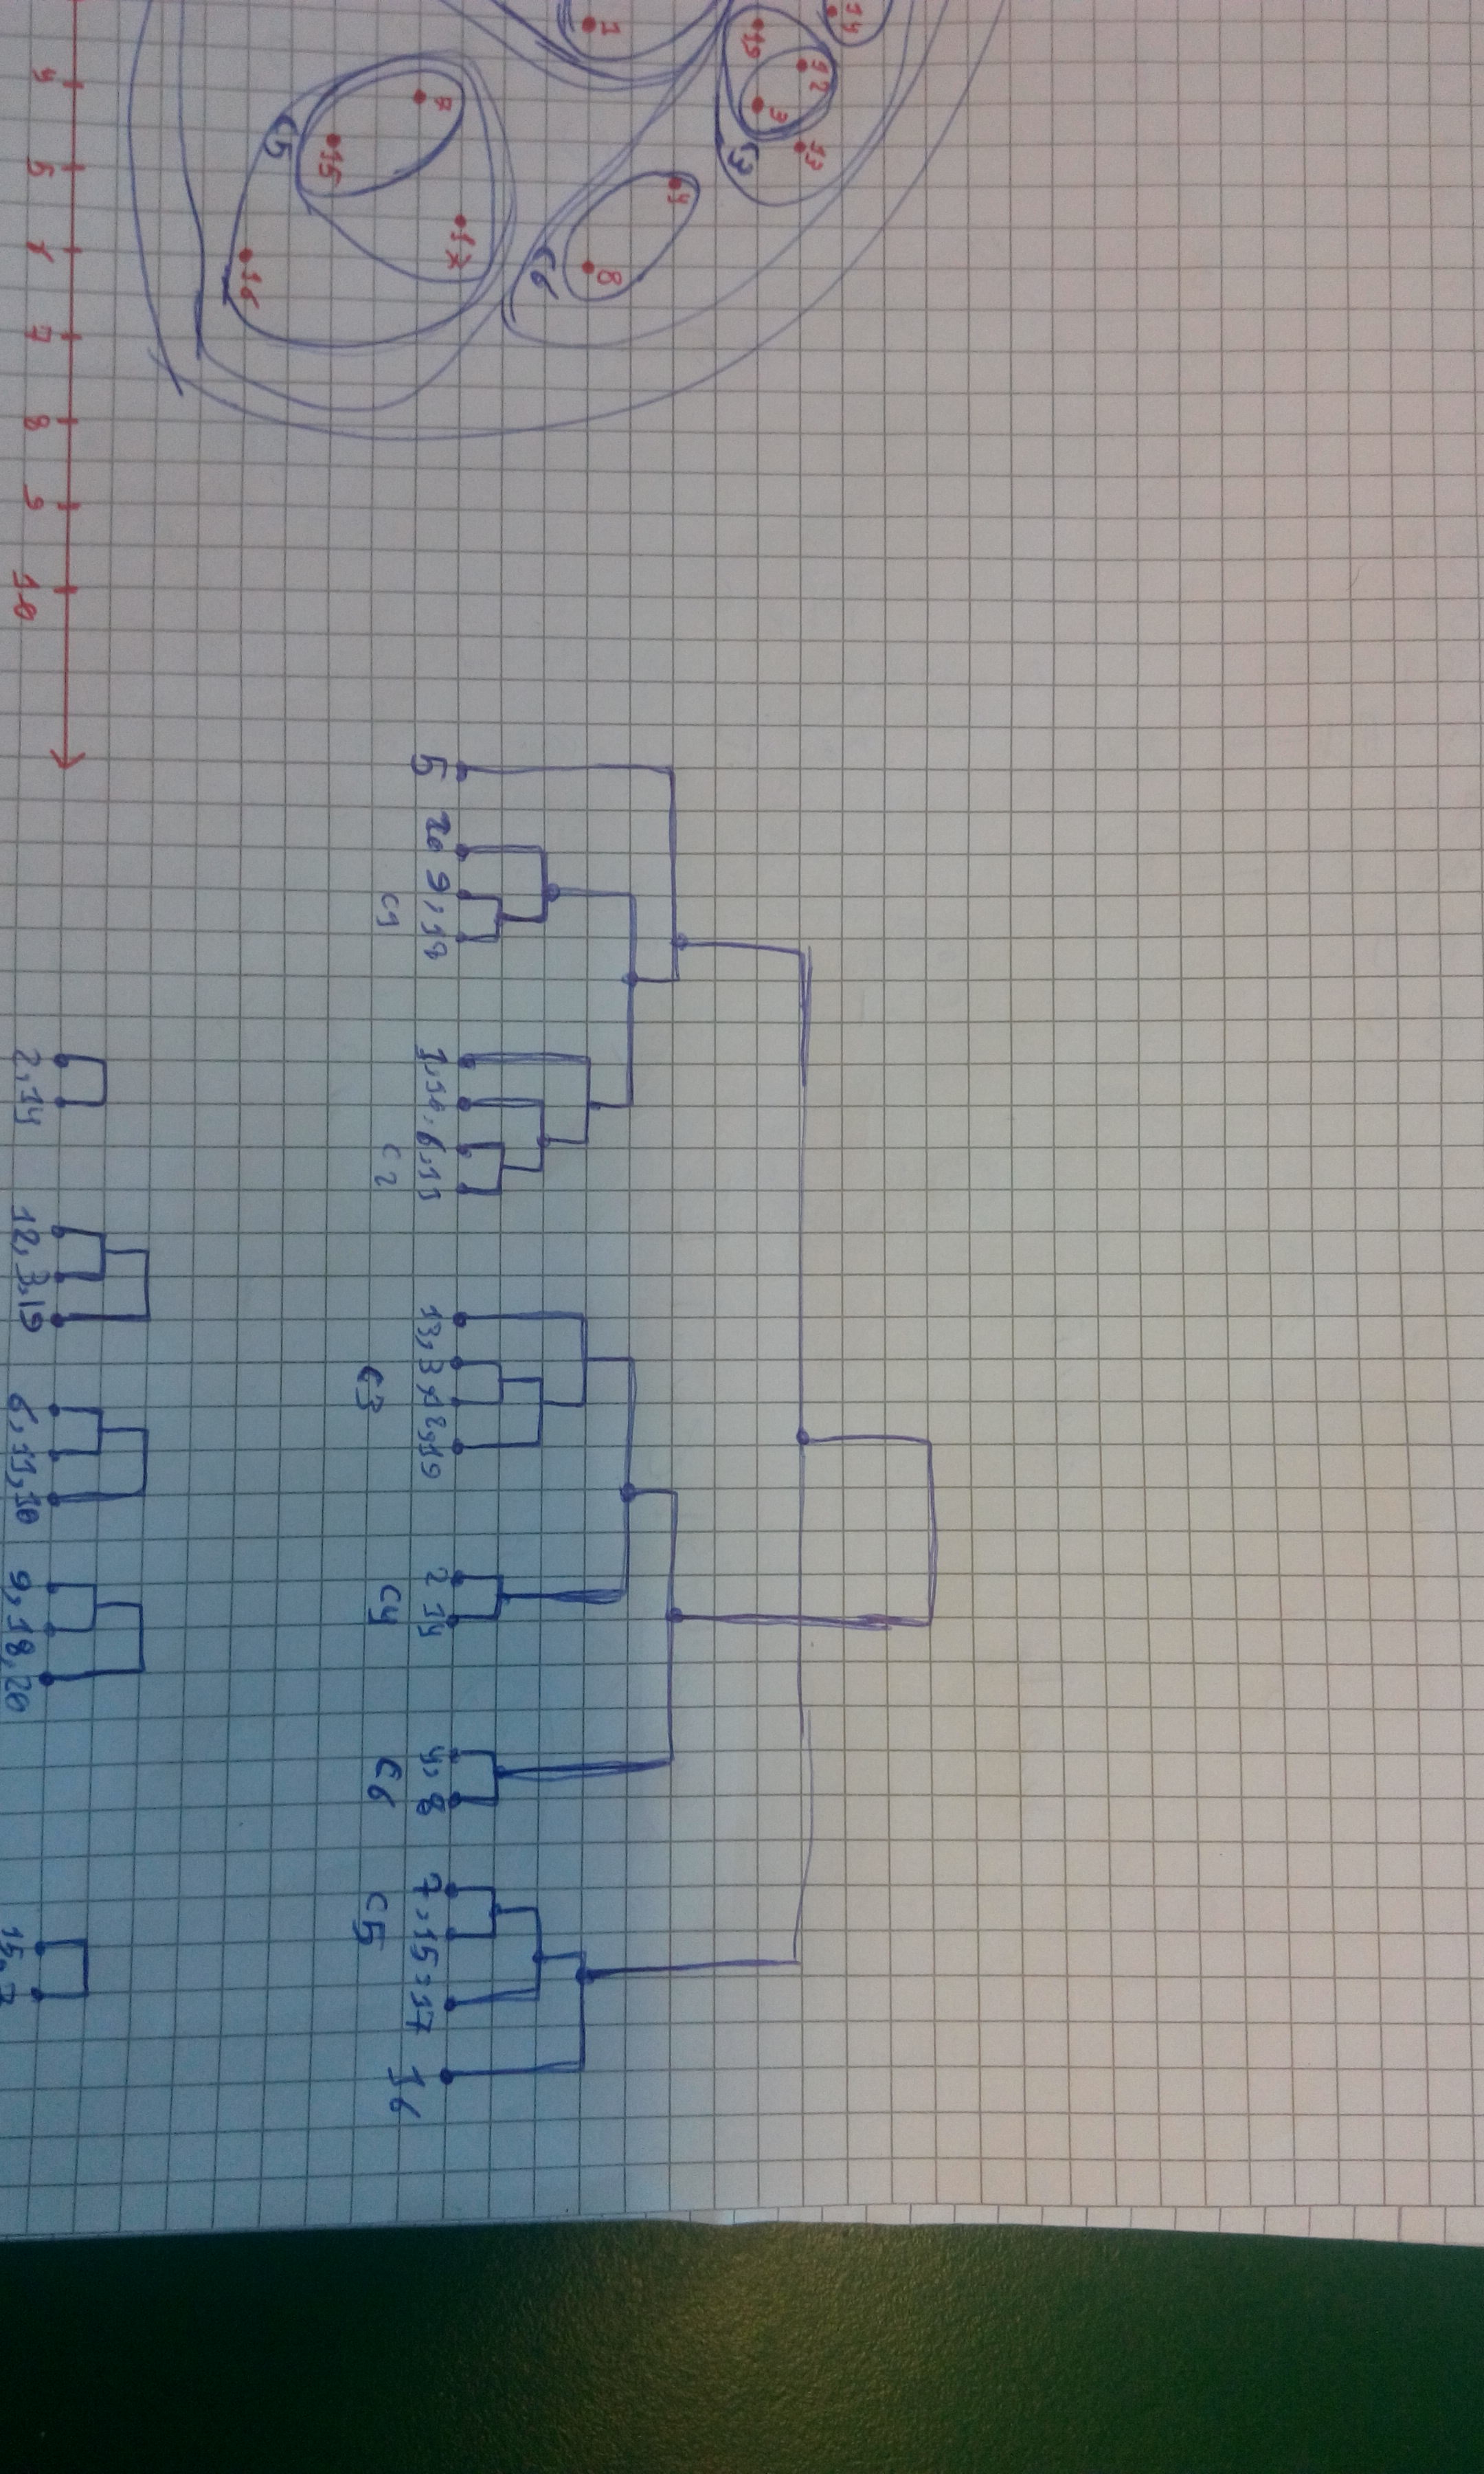
\includegraphics[angle=90,scale=0.23,trim={15cm 15cm 25cm 37cm},clip]{complete_tree.jpg}
\caption{The tree}
\end{figure}
\section*{Third Question}
For this question I wrote a python code,
\begin{enumerate}
\item  First calculate the distance between the four centers and assign the point to the closest center.
\item Plot the data
\item Calculate the new centers 
\item Repeat
\end{enumerate} Here it is : 
\begin{lstlisting}[language=Python]
import pandas as pd
import numpy as np
#%matplotlib inline
import matplotlib.pyplot as plt
from IPython.display import display, HTML
from mpl_toolkits.mplot3d import Axes3D
from matplotlib import cm
from operator import attrgetter
from matplotlib.patches import Ellipse
from math import atan2,degrees
import numpy.random as rnd

points = pd.read_csv('Clustering.csv',sep=',')

class CenterValue:
    def __init__ (self,p,val,lab):
        self.value=val
        self.point=p
        self.label=lab
    def __str__(self):
        return 'point:{},Value:{},index:{}'.format(self.point,self.value,self.label)

def Distance(p1,p2indx):
    p1 = np.array(p1)
    p2 = np.array((points.X[p2indx],points.Y[p2indx]))
    return np.linalg.norm(p1-p2)

def K_mean(centerpoints):
    centers={}
    for i in centerpoints:
        centers[i]=[]
    for i in range(len(points.index)):
        values=[]
        values.append(CenterValue(centerpoints[0],Distance(centerpoints[0],i),i))
        values.append(CenterValue(centerpoints[1],Distance(centerpoints[1],i),i))
        values.append(CenterValue(centerpoints[2],Distance(centerpoints[2],i),i))
        values.append(CenterValue(centerpoints[3],Distance(centerpoints[3],i),i))
        values.sort(key=lambda x: x.value, reverse=False)
        centers[values[0].point].append(GetPointsList([i])[0])
    return centers     

def GetPointsList(Indexs):
    lst=[]
    for i in Indexs:
        lst.append((points.X[i],points.Y[i]))
    return lst

def Get_Means(dictionary_of_lists):
    lst=[]
    for i in dictionary_of_lists.keys():
        mX=0
        mY=0
        for p in dictionary_of_lists[i]:
            mX+=p[0]
            mY+=p[1]
        lst.append((mX/len(dictionary_of_lists[i]),mY/len(dictionary_of_lists[i])))
    return lst

def Plot(k):
    keys = k.keys()
    fig = plt.figure(0)
    ax = fig.add_subplot(111, aspect='equal')
    ax.plot([t[0] for t in k[keys[0]]], [t[1] for t in k[keys[0]]], 'rs')
    ax.plot([t[0] for t in k[keys[1]]], [t[1] for t in k[keys[1]]], 'bs')
    ax.plot([t[0] for t in k[keys[2]]], [t[1] for t in k[keys[2]]], 'gs')
    ax.plot([t[0] for t in k[keys[3]]], [t[1] for t in k[keys[3]]], 'ms')
    for k in keys:
        ax.plot(k[0],k[1],'k*')
        ax.annotate('Cntr',(k[0],k[1]))
    ax.axis([0, 10, 0,10])
    plt.show()

#First Iteration
k = K_mean(GetPointsList(range(4)))
Plot(k)

#Each Time new Iteration
k = Get_Means(k)
k = K_mean(k)
Plot(k)
\end{lstlisting}
The previous code output the following : 
\begin{figure}[H]
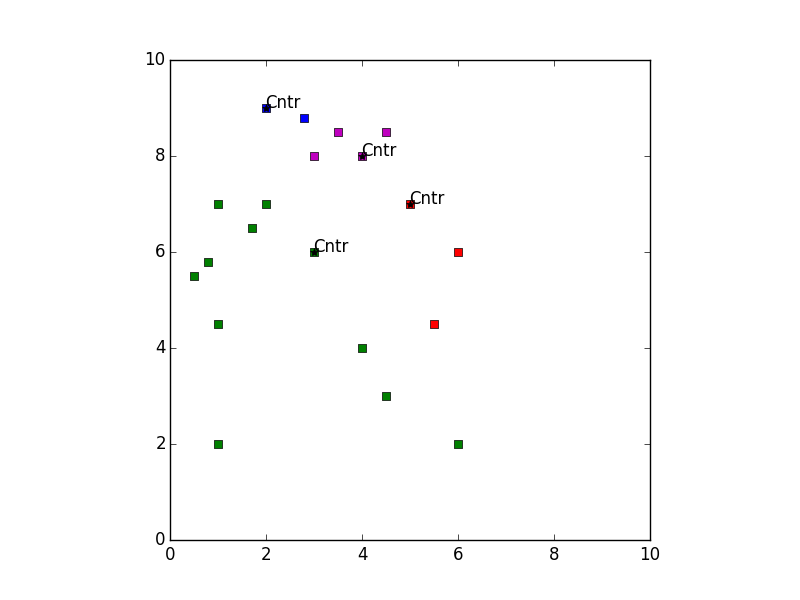
\includegraphics[scale=0.5,trim={3cm 1cm 3cm 1cm},clip]{1.png}
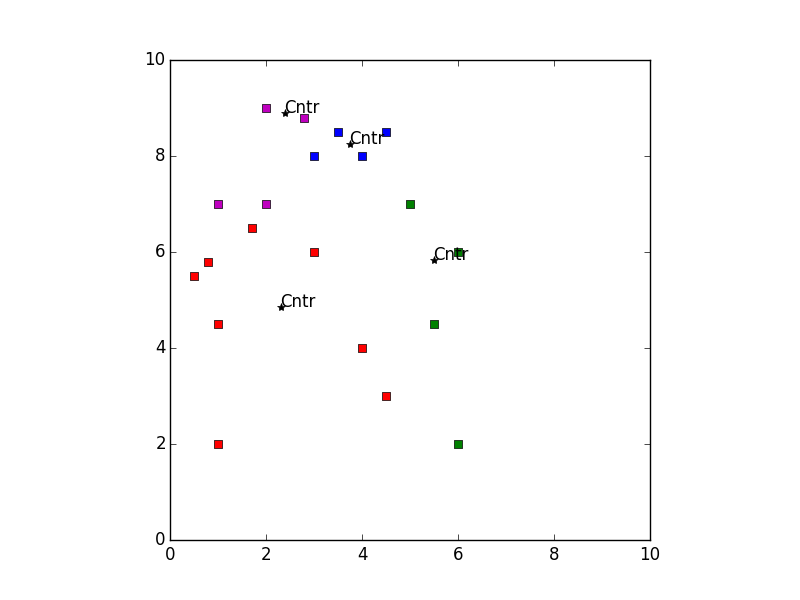
\includegraphics[scale=0.5,trim={3cm 1cm 3cm 1cm},clip]{2.png}\\
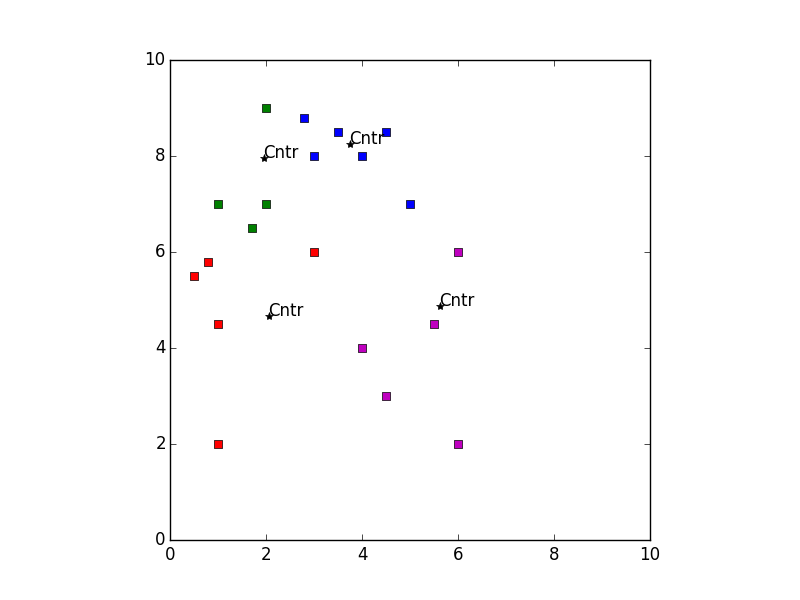
\includegraphics[scale=0.5,trim={3cm 1cm 3cm 1cm},clip]{3.png}
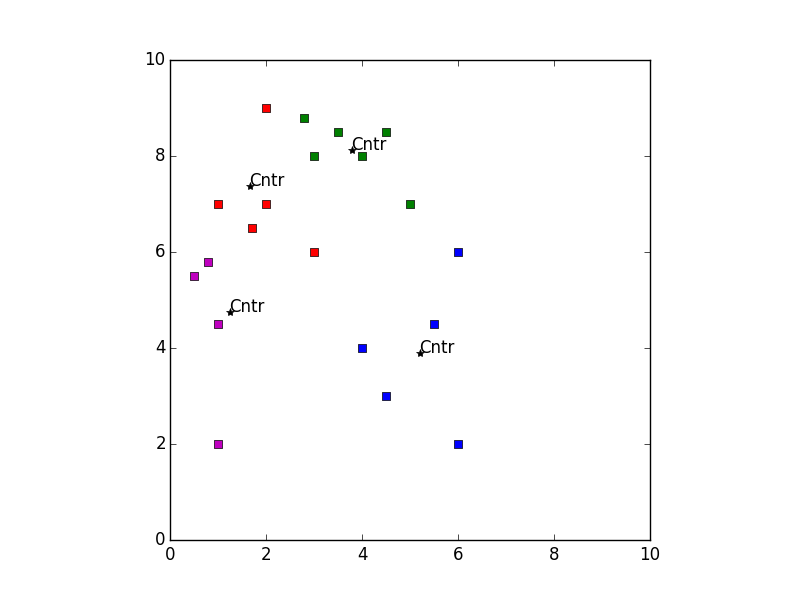
\includegraphics[scale=0.5,trim={3cm 1cm 3cm 1cm},clip]{4.png}\\
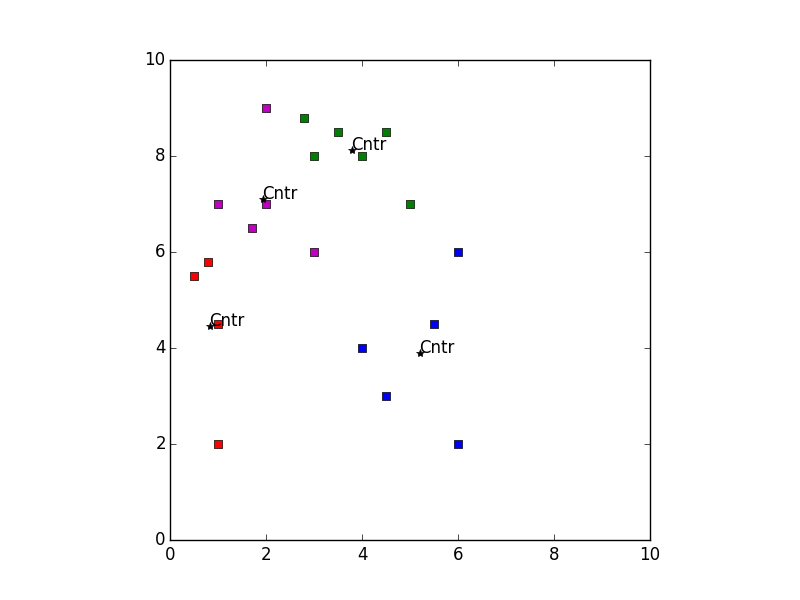
\includegraphics[scale=0.5,trim={3cm 1cm 3cm 1cm},clip]{5.png}
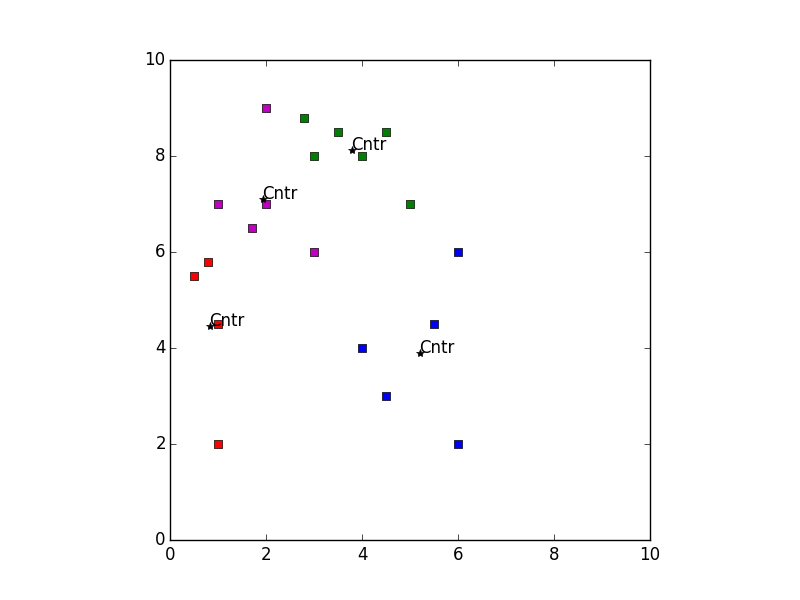
\includegraphics[scale=0.5,trim={3cm 1cm 3cm 1cm},clip]{6.png}\\
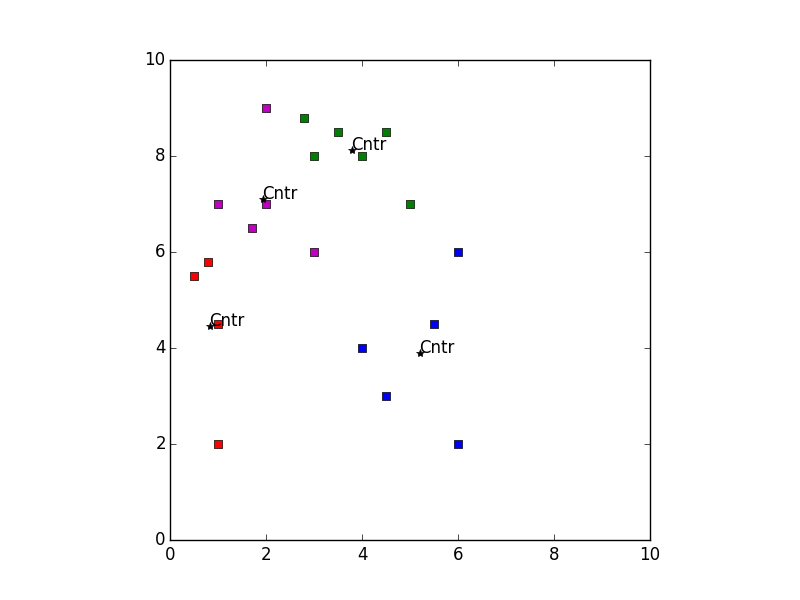
\includegraphics[scale=0.5,trim={3cm 1cm 3cm 1cm},clip]{7.png}
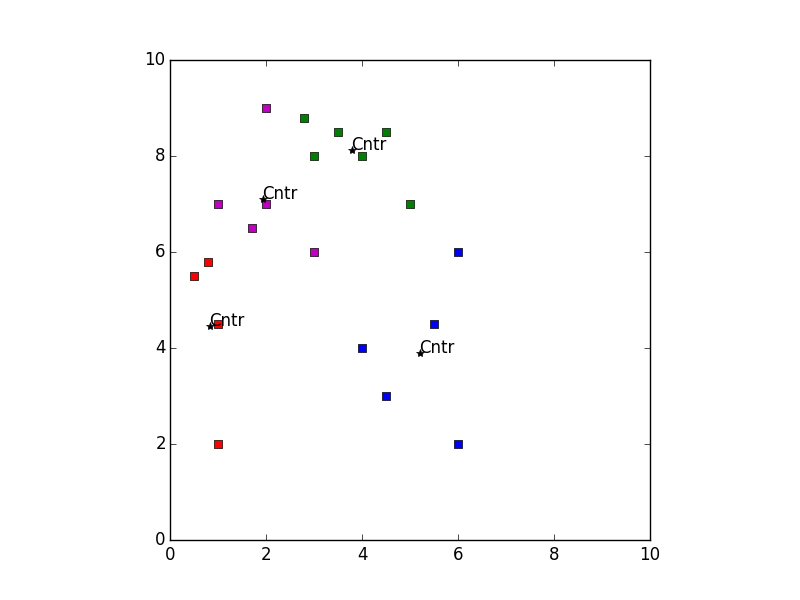
\includegraphics[scale=0.5,trim={3cm 1cm 3cm 1cm},clip]{8.png}
\caption{Shows how centers change counting(1,2),(3,4)}
\end{figure}
In the previous figures we can see that after the 5th iteration the centers got stable 
\section*{Fourth Question}
The Slide already added.
\section*{Fifth Question}
\href{https://www.kaggle.com/dsoreo/home-depot-product-search-relevance/testing-r/notebook}{Analysis}\\
To Find something different than the previous information I stemmed the text using the following code :
\begin{lstlisting}[language=Python]

# coding: utf-8

# In[1]:

import time
start_time = time.time()

import numpy as np
import pandas as pd
from nltk.stem.porter import *
stemmer = PorterStemmer()
#from nltk.stem.snowball import SnowballStemmer #0.003 improvement but takes twice as long as PorterStemmer
import re
import random
random.seed(1301)


# In[2]:

df_train = pd.read_csv('Data Warehouse/train.csv', encoding="ISO-8859-1")
df_test = pd.read_csv('Data Warehouse/test.csv', encoding="ISO-8859-1")
df_pro_desc = pd.read_csv('Data Warehouse/product_descriptions.csv')
df_attr = pd.read_csv('Data Warehouse/attributes.csv', encoding="ISO-8859-1")
df_brand = df_attr[df_attr.name == "MFG Brand Name"][["product_uid", "value"]].rename(columns={"value": "brand"})
num_train = df_train.shape[0]
df_all = pd.concat((df_train, df_test), axis=0, ignore_index=True)
df_all = pd.merge(df_all, df_pro_desc, how='left', on='product_uid')
df_all = pd.merge(df_all, df_brand, how='left', on='product_uid')


# In[3]:

def stem_sentence(sentence):
    sentence = [stemmer.stem_word(x) for x in sentence.split()]
    return sentence


# In[4]:

df_all['search_term'] = df_all['search_term'].map(lambda x:stem_sentence(x))
df_all['product_title'] = df_all['product_title'].map(lambda x:stem_sentence(x))
df_all['product_description'] = df_all['product_description'].map(lambda x:stem_sentence(x))


# In[9]:

words={}
def AddToWords(sentence):
    for i in sentence:
        words[i]=True


# In[10]:

df_all['search_term'] = df_all['search_term'].map(lambda x:AddToWords(x))
df_all['product_title'] = df_all['product_title'].map(lambda x:AddToWords(x))
df_all['product_description'] = df_all['product_description'].map(lambda x:AddToWords(x))


# In[11]:

len(words.keys())
\end{lstlisting} 
The Total number of distinct words is : 
\textbf{Note:}All code,pythhon ,tex,pdf,etc... files exist in \href{https://github.com/aqeel13932/DM/tree/master/HW11}{github}
\begin{center}
\textbf{E.O.F}
\end{center}
\end{document}